\subsubsubsection{arithmetic\_extension}

\hspace*{\fill}

\indent To understand the design principle of this Gate, we must first understand \href{https://en.wikipedia.org/wiki/Field_extension#Extension_field}{field extensions}. 

Taking Plonky2's Goldilocks field as an example, we give the extension field elements under quadratic, quartic, and quintic extensions respectively in \figref{fig:goldilocks field extension}.

\begin{figure}[!ht]
    \centering
    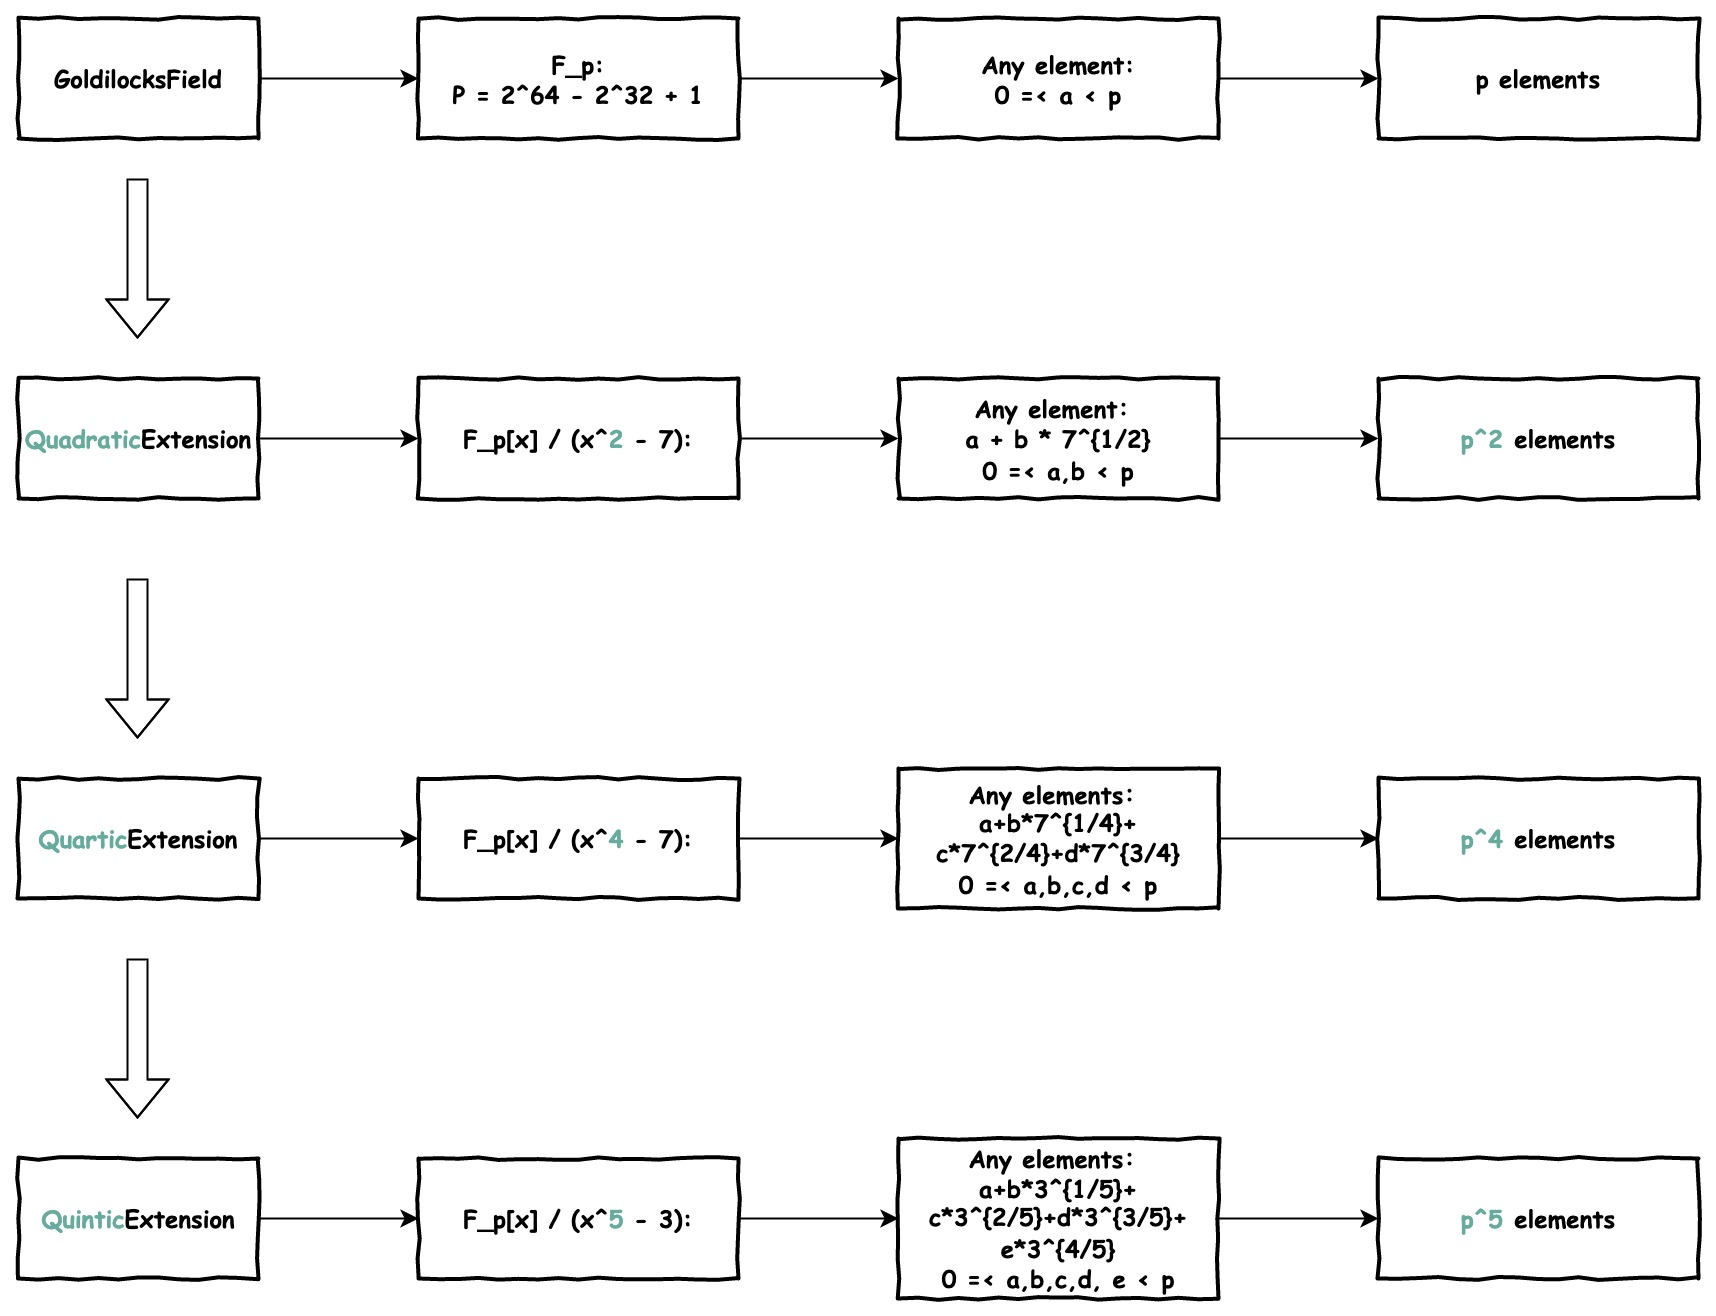
\includegraphics[width=0.6\textwidth]{gates/arthmetic_extension_ext.jpeg}
    \caption{Goldilocks Field Extension}
    \label{fig:goldilocks field extension}
\end{figure}

It is easy to see that for quadratic extension field, the elements on its domain take the form $a+b\sqrt{7}, \ a,b \in \mathbb{F}_p$.
It can be seen that on the quadratic extension field, there are $p^2$ elements and the original field is a subset of the quadratic extension field.

ArithmeticExtensionGate is also a gate that can perform a weighted multiply-add, i.e.
\[ \text{res} = \text{cons\_0} \times \text{mul\_0} \times \text{mul\_1} + \text{cons\_1} \times \text{add} \]

The elements of the QuadraticExtension Field are represented in the form $[a, b]$, so the Gate design for arithmetic\_extension has the following form:

The structure of the gate is shown in \figref{fig:arthmetic-extension}. There's only one constraint per operation, and the degree is 3.
\begin{figure}[!ht]
    \centering
    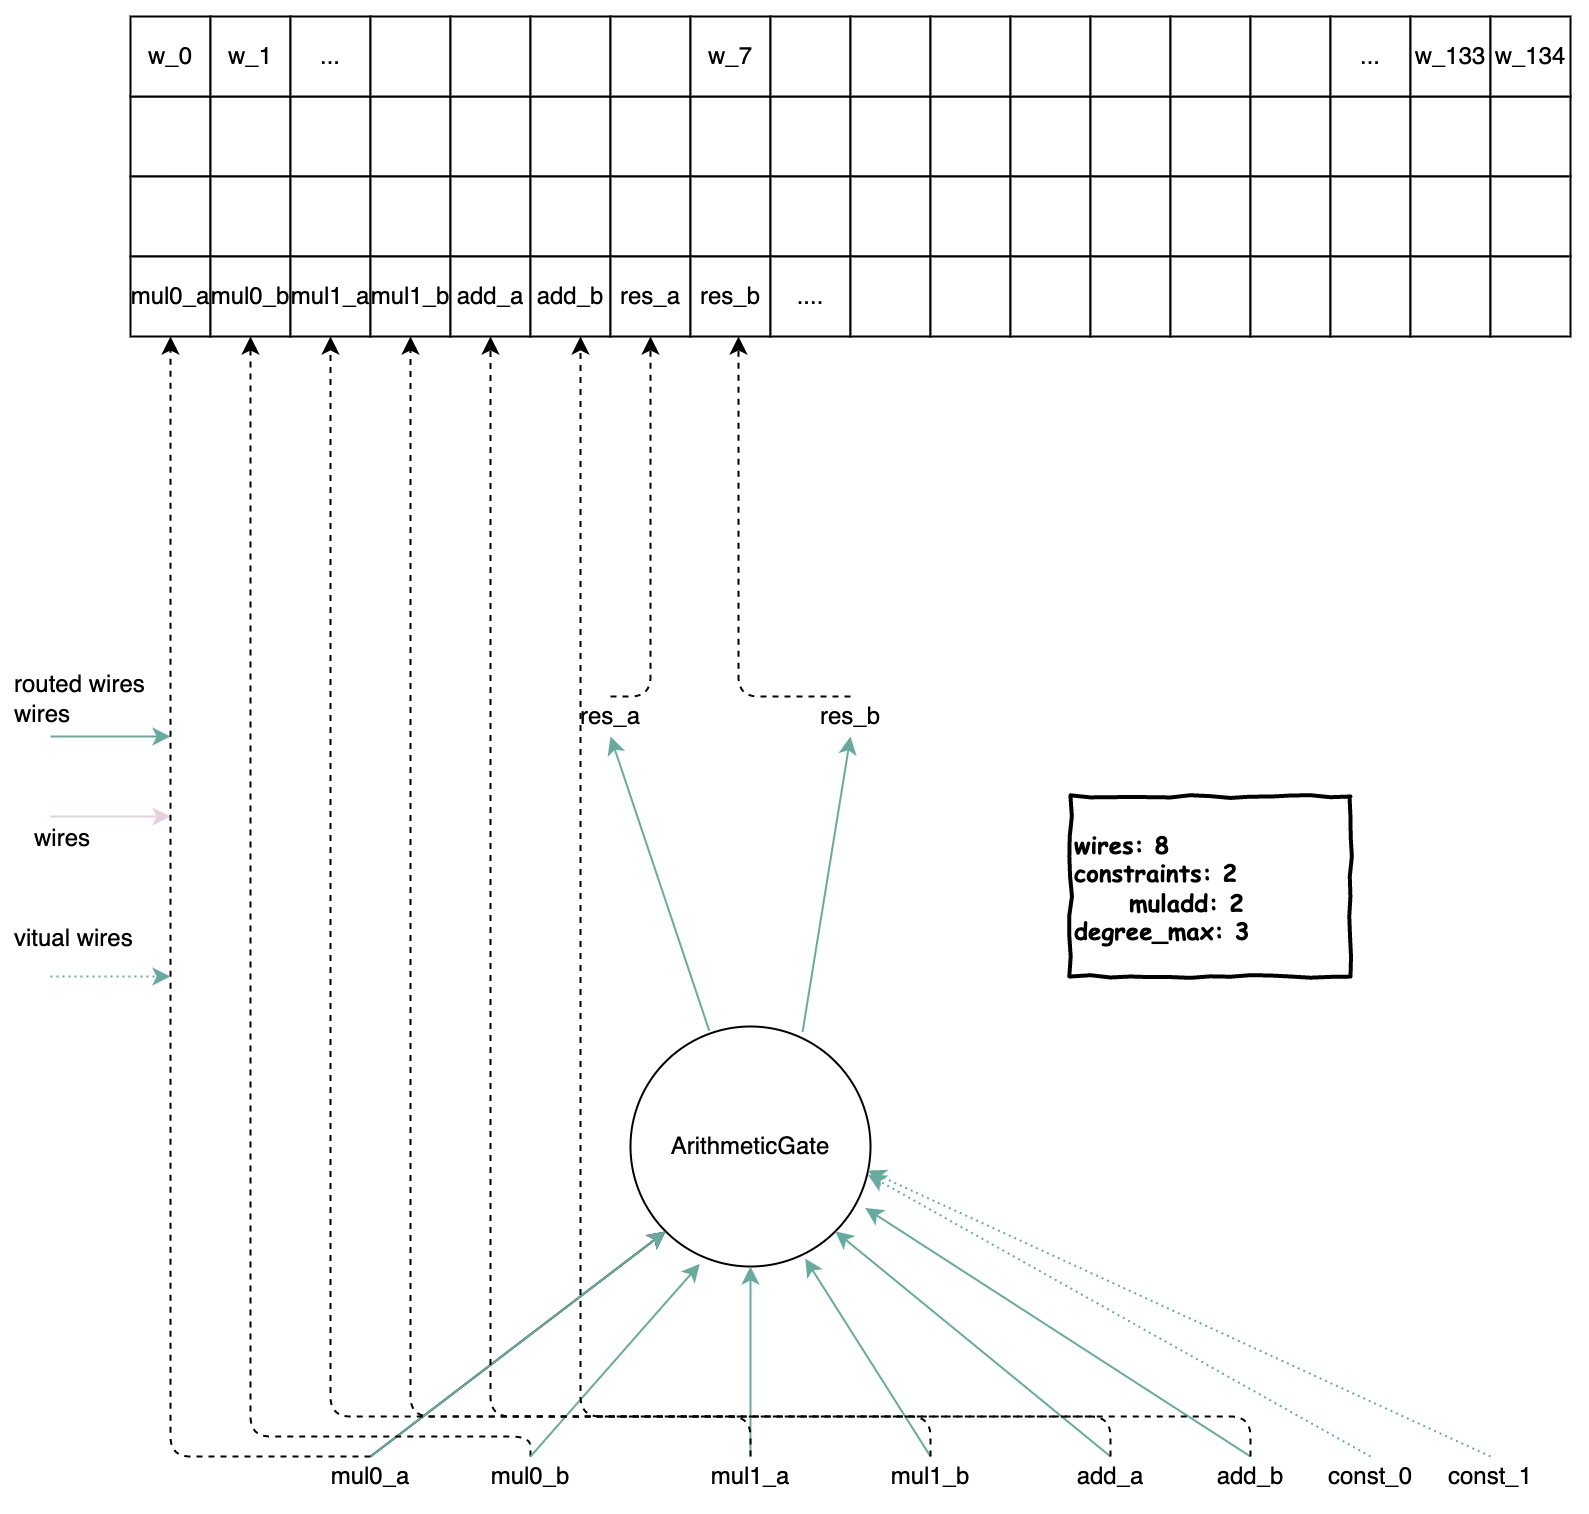
\includegraphics[width=0.6\textwidth]{gates/arthmetic_extension.jpeg}
    \caption{ArithmeticExtensionGate}
    \label{fig:arthmetic-extension}
\end{figure}
